\section{Elo Rating System}
\label{Elo}
The Elo rating system is a method for ranking competitors that is used in Chess and many similar competitor-versus-competitor games. It works by predicting a win-rate of the competitors and then changing the rating according to what the likelihood of the outcome is - if a competitor with a low expected win rate loses, Elo loss is low; however, if that same competitor would win, Elo gain would be very high. Below are the formulae used for our implementation:\\

\noindent The expected winrate of a Script $A$ against a Script $B$ is \\

{\Large\centerline{$E_{A} = \frac{1}{1 + 10^\frac{R_{B}-R_{A}}{400}}$}} \vspace{2mm}

\hspace*{5mm} where $R_{A}$ and $R_{B}$ are the Elo ratings of Script $A$ and Script $B$, respectively.\\

\noindent The resulting rating change of a Script $X$ with an expected winrate $E_{X}$ is \\

{\Large\centerline{$R_{X}' = R_{X} + 32(W - E_{X})$}} \vspace{2mm}

\hspace*{5mm} where $R_{X}$ is the old rating of $X$, $R_{X}'$ is the new updated rating \\
\hspace*{17mm} and $W$ is a value $1$ or $0$ if $X$ wins or loses, respectively.\\

All scripts begin with an $R_{X}$ of 1400.  For games with more than two racers, each racer `wins' against anyone they finish ahead of, and `loses' to anyone they finish behind. $E_{X}$ is calculated against each script. For example, in a 3-way race, the 2\textsuperscript{nd} place finisher loses Elo as if it had lost a head-to-head race with the 1\textsuperscript{st} place script, but gains Elo as if it had defeated the 3\textsuperscript{rd} place script in a head-to-head. Depending on the ratings of the scripts at the start of the race, this script could have a net positive or negative Elo change.

\section{Example AI Scripts}
In this section there are several examples of AI scripts that our system supports. Our most basic script, StayLeft[\ref{jsbasic}], instructs the car to maintain a constant speed (lines 7, 9) and hug the left edge of the road (line 4). A functionally equvilant script, StayLeft (Events)[\ref{jsevents}], shows how the Event API can be used to simplify such scripts. 

A more fleshed out example, Rambo[\ref{rambo}], highlights  the depth advanced users can reach. Rambo maintains a high speed but breaks when approaching a corner (line 34). If Rambo is far from the next corner it will activate the Boost function, throwing it forward (line 22). Rambo will also hug the inside lane as it drives around the track (lines 27, 29). Finally, Rambo will try to attack overtaking cars. For example, if a car is approaching on the left, rambo will increase in speed and swerve left (lines 5, 12). If a car is directly in front, Rambo will no longer slow down for corners and will instead Boost the enemy off the track (line 15). Rambo (CoffeeScript)[\ref{coffeerambo}] shows how the same behaviour can be specified in CoffeeScript.


\subsection{StayLeft}
\label{jsbasic}
\begin{figure}[H]
\begin{lstlisting}[language=JavaScript]
var maxSpeed = 18;

var PhysicsUpdate = function(api) {
    api.ChangeLaneLeft();
    
    if(api.GetSpeed() > maxSpeed) {
        api.SetThrottle(0);
    } else {
        api.SetThrottle(70);
    }
};
\end{lstlisting}
\end{figure}

\subsection{StayLeft (Events)}
\label{jsevents}
\begin{figure}[H]
\begin{lstlisting}[language=JavaScript]
var maxSpeed = 18;

When.SpeedLessThan(maxSpeed).SetThrottle(70);
When.SpeedMoreThan(maxSpeed).SetThrottle(0);

var PhysicsUpdate = function(api) {
    api.ChangeLaneLeft();
};
\end{lstlisting}
\end{figure}

\subsection{Rambo (JavaScript)}
\label{rambo}
\begin{figure}[H]
\begin{lstlisting}[language=JavaScript]
var NORMAL_SPEED  = 22;
var RAMMING_SPEED = 30;
var maxSpeed = NORMAL_SPEED; 

var Ram = function(api) { maxSpeed = RAMMING_SPEED; };

var StopRam = function(api) { maxSpeed = NORMAL_SPEED; };

When.CarOnRight().Then(Ram).ChangeLaneRight()
    .After(100).Then(StopRam).ChangeLaneLeft();
    
When.CarOnLeft().Then(Ram).ChangeLaneLeft()
    .After(100).Then(StopRam).ChangeLaneRight();
    
When.CarInFront().Then(Ram).Boost()
    .After(100).Then(StopRam);

var PhysicsUpdate = function(api) { 
    var distance = api.GetDistanceToNextCorner(); 
    
    if (distance > 85) { 
        api.Boost(); 
    }
    
    if (maxSpeed != RAMMING_SPEED) {
       if (api.GetNextCornerAmount() < 0) { 
            api.ChangeLaneLeft(); 
        } else { 
            api.ChangeLaneRight(); 
        } 
    }
    
    if (api.GetSpeed() > 22 && distance < 40 && !api.CarInFront()) { 
        api.SetThrottle(-50); 
    } else if (api.GetSpeed() > maxSpeed && !api.CarInFront()) { 
        api.SetThrottle(0); 
    } else {
        api.SetThrottle(100);
    }
};
\end{lstlisting}
\end{figure}
\subsection{Rambo (CoffeeScript)}
\label{coffeerambo}
\begin{figure}[H]
\begin{lstlisting}[language=JavaScript]
NORMAL_SPEED  = 22
RAMMING_SPEED = 30
maxSpeed = NORMAL_SPEED

Ram     = (api) -> maxSpeed = RAMMING_SPEED
StopRam = (api) -> maxSpeed = NORMAL_SPEED

When.CarOnRight().Then(Ram).ChangeLaneRight()
    .After(100).Then(StopRam).ChangeLaneLeft()
    
When.CarOnLeft().Then(Ram).ChangeLaneLeft()
    .After(100).Then(StopRam).ChangeLaneRight()
    
When.CarInFront().Then(Ram).Boost()
    .After(100).Then(StopRam)

PhysicsUpdate = (api) -> 
    distance = api.GetDistanceToNextCorner() 
    
    if distance > 85
        api.Boost(); 

    if maxSpeed != RAMMING_SPEED 
        if api.GetNextCornerAmount() < 0 
            api.ChangeLaneLeft() 
        else
            api.ChangeLaneRight()
    
    if api.GetSpeed() > 22 and distance < 40 and api.CarInFront() 
        api.SetThrottle(-50) 
    else if api.GetSpeed() > maxSpeed and !api.CarInFront() 
        api.SetThrottle(0) 
    else
        api.SetThrottle(100)
\end{lstlisting}
\end{figure}

\section{Instruction Manual (Handout)}

\begin{figure}[H]
\centering
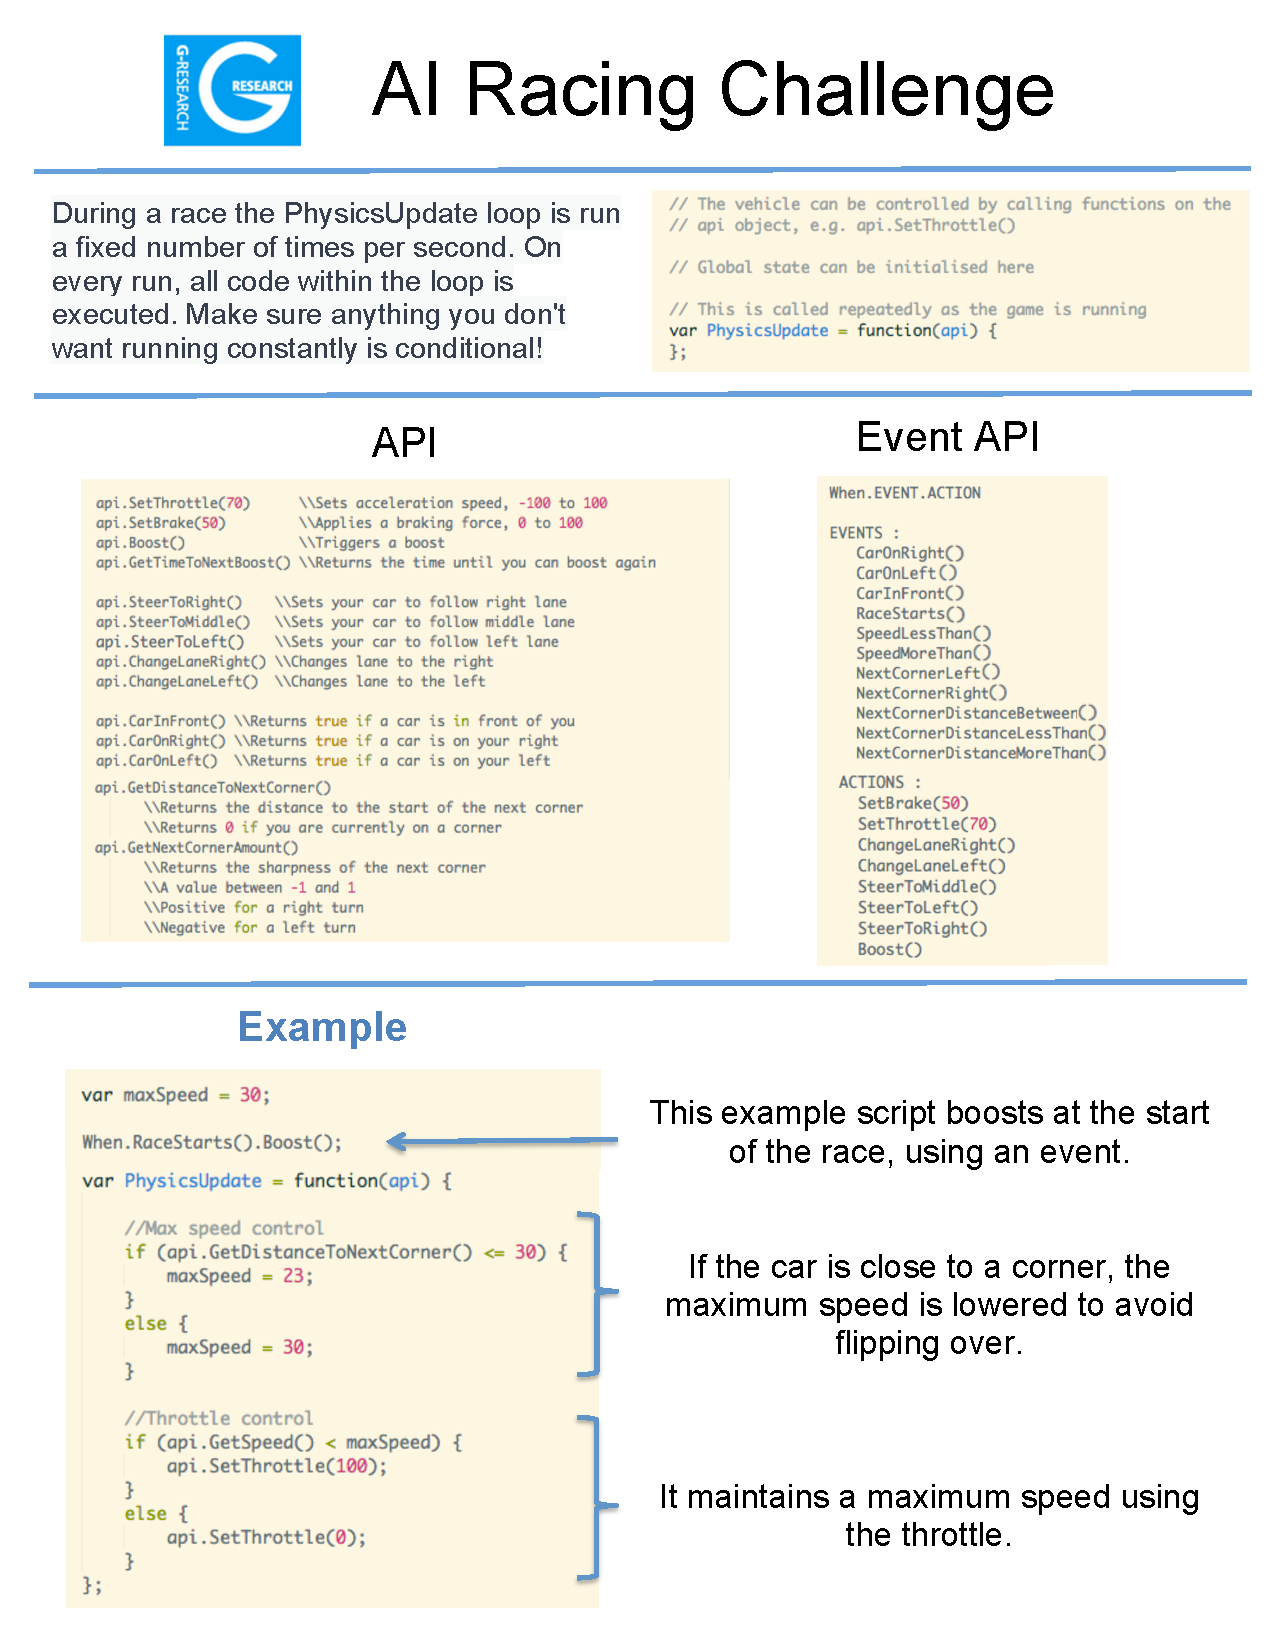
\includegraphics[width=\textwidth,page=1]{Handout.pdf}
\caption{Handout - first page.}
\end{figure}
\begin{figure}[H]
\centering
\includegraphics[width=\textwidth,page=2]{Handout.pdf}
\caption{Handout - second page.}
\end{figure}

\section{Development Process}

\begin{figure}[H]
\centering
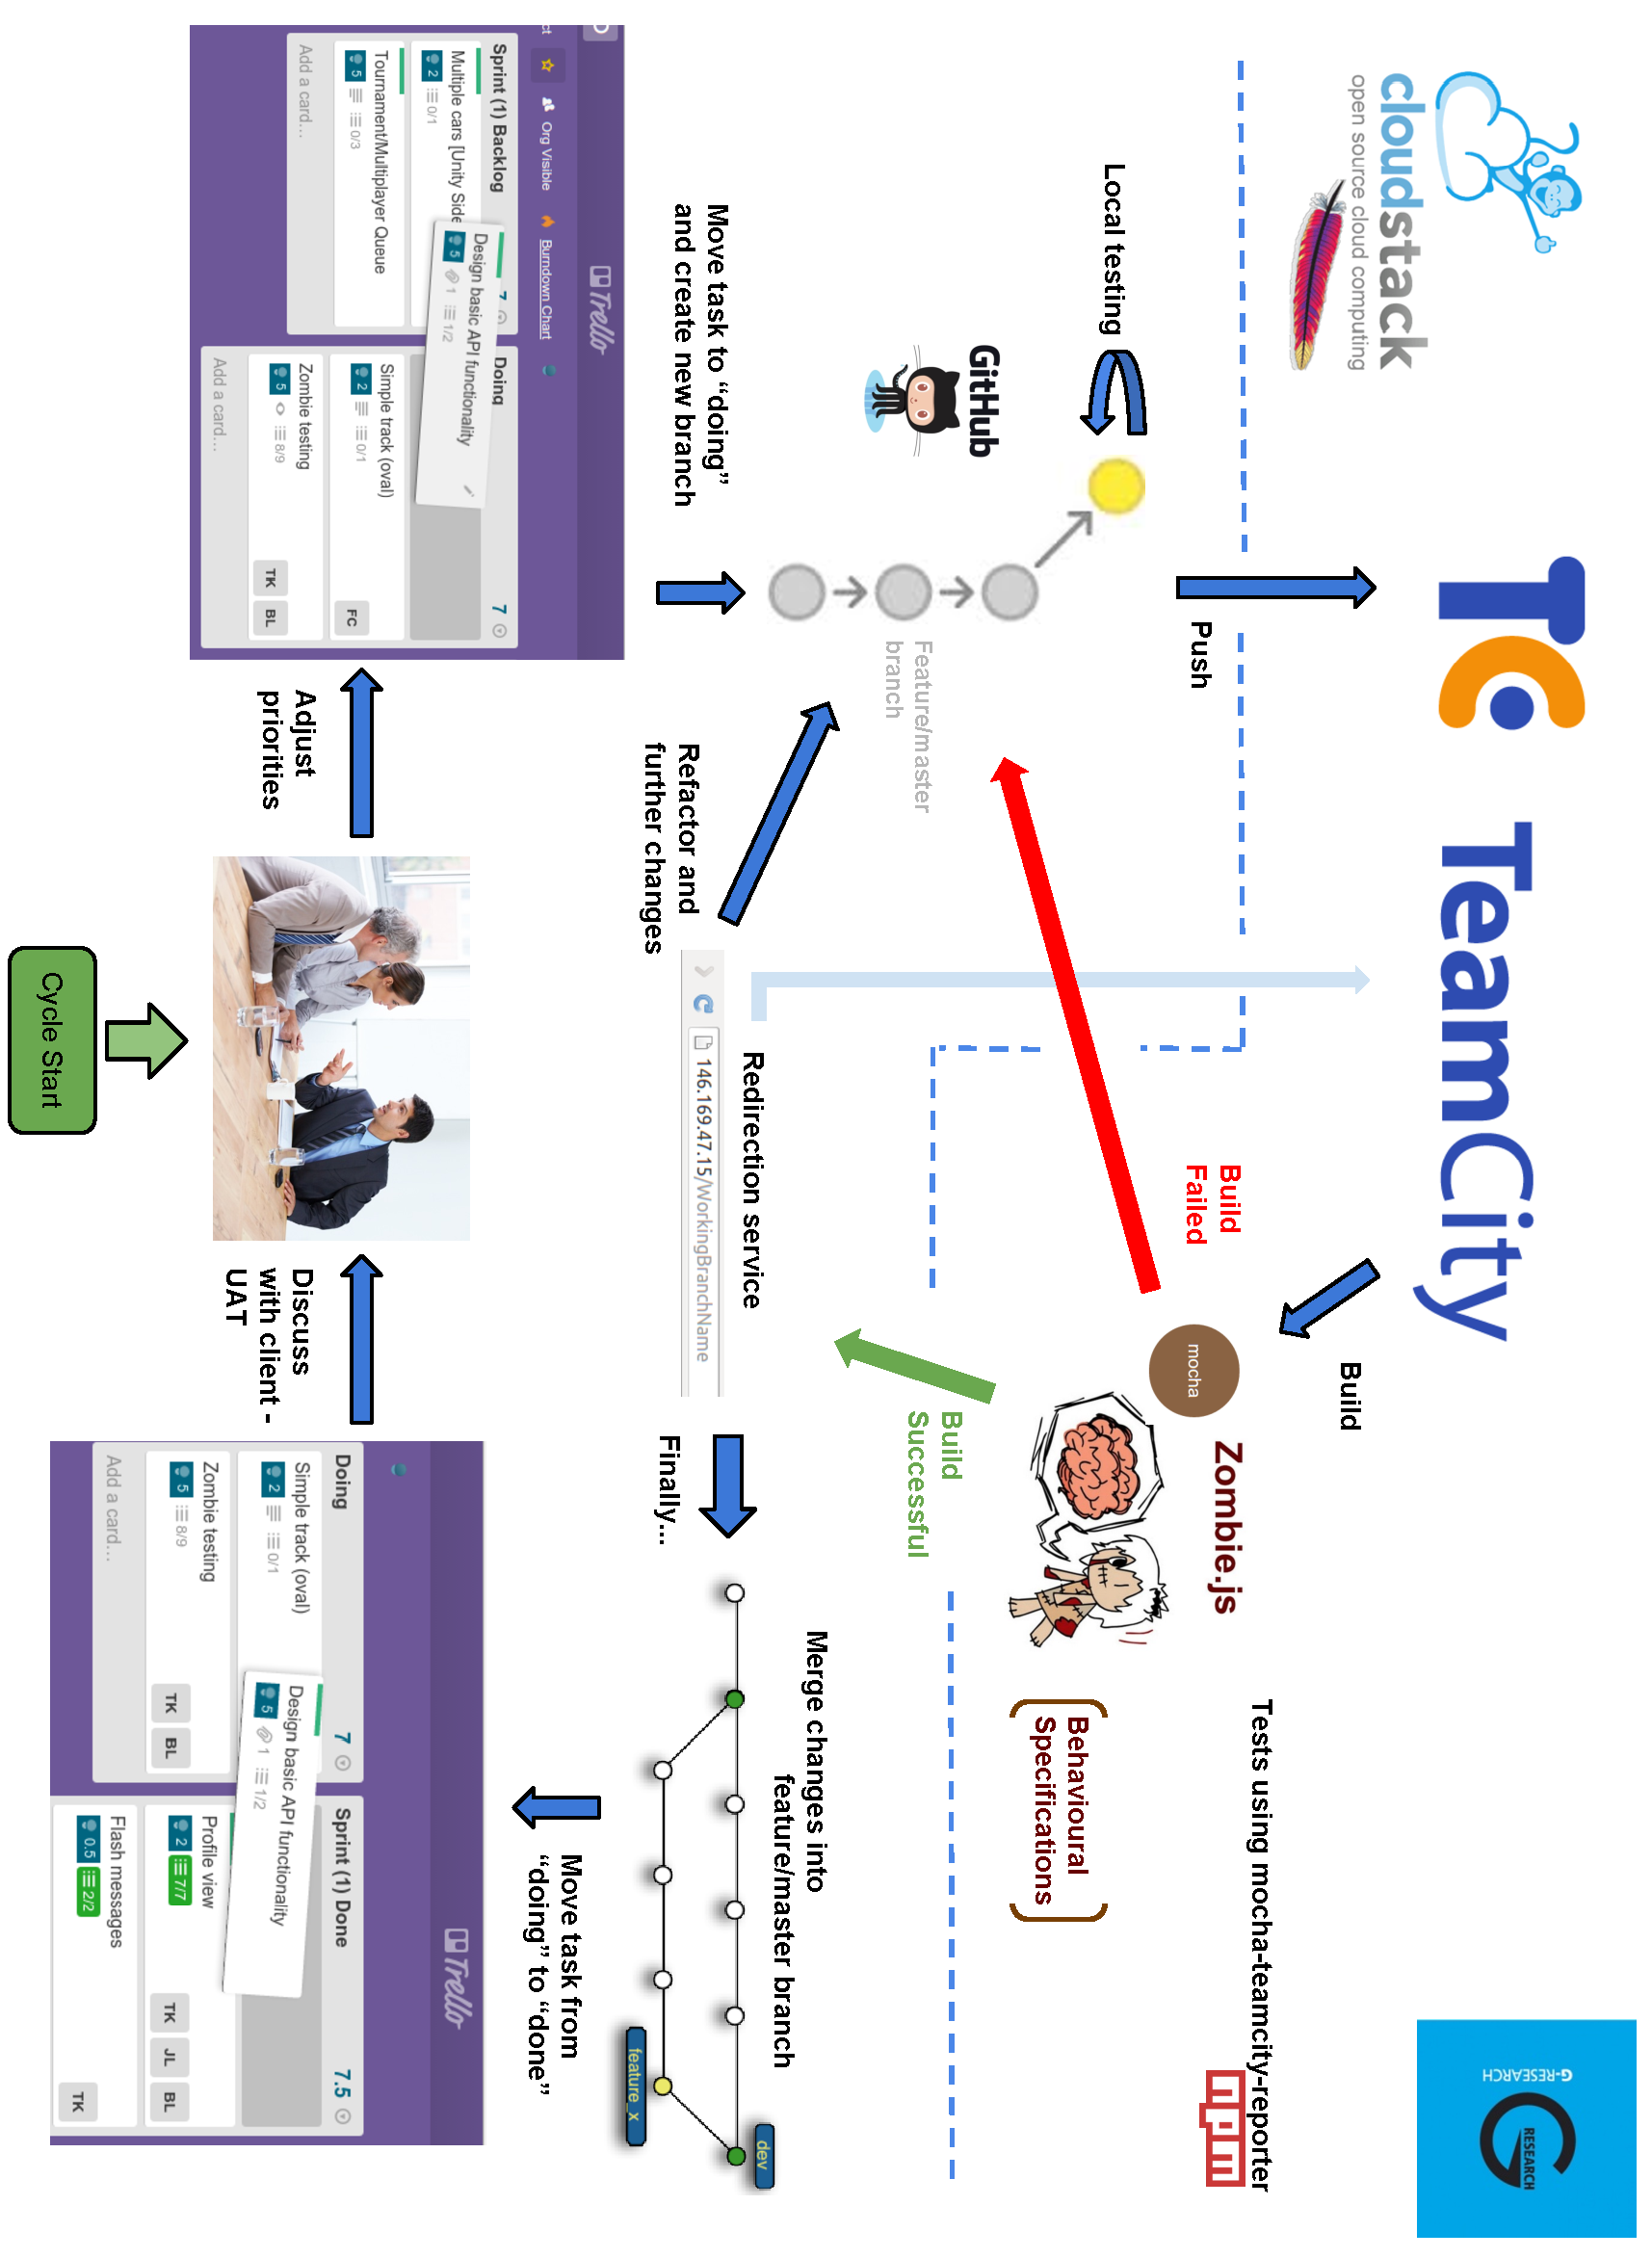
\includegraphics[width=\textwidth]{DevProcess.pdf}
\caption{Development process diagram.}
\end{figure}